% Created 2023-03-31 vie 21:31
% Intended LaTeX compiler: pdflatex
\documentclass[a4paper]{llncs}
\usepackage[hidelinks]{hyperref}
\usepackage[utf8]{inputenc}
\usepackage[T1]{fontenc}
\usepackage{graphicx}
\usepackage{longtable}
\usepackage{wrapfig}
\usepackage{rotating}
\usepackage[normalem]{ulem}
\usepackage{amsmath}
\usepackage{amssymb}
\usepackage{capt-of}
\usepackage{hyperref}
\usepackage{listings}
\usepackage[spanish, american]{babel}
\usepackage{graphicx}
\usepackage[spanish]{cleveref}
\usepackage{multirow}
\usepackage[]{inputenc}
\usepackage[style=apa]{biblatex} % Bibliography
\addbibresource{./bib/referencias.bib}
\usepackage{csquotes}
\usepackage{multirow}
\usepackage{graphicx}
\voffset=10mm
\hoffset=-3.5mm
\widowpenalty=9999
\clubpenalty=9999
\hyphenpenalty=500
\exhyphenpenalty=500
\pagestyle{empty}
\date{\today}
\title{Paper Comia 23}
\begin{document}




\selectlanguage{spanish}
  \title{Pseudoetiquetado para el análisis de polaridad en tuits: un primer
    acercamiento}
  % \author{}
  % \institute{}
  % \author{Diana Jimenez, Marco A. Cardoso-Moreno, Cesar Macias}
  % \authorrunning{Jimenez et al.}


  % \institute{Instituto Politécnico Nacional, \\ Centro de Investigación en Computación, \\
  %   Laboratorio de Ciencias Cognitivas Computaciones, Ciudad de México, México \\
  %   \email{\{correo_blue,mcardosom2021,correo_cesar\}@cic.ipn.mx}}

  \maketitle

\begin{abstract}
El análisis de polaridad es un tema de creciente interés, sobre todo en redes
sociales ya que permite conocer si la opinión de las personas es negativa o
positiva respecto a un tema en particular, en un ambiente libre; lo que nos
permite conocer el impacto de productos, noticias, etc. En este trabajo se
realiza análisis de polaridad en tuits en español haciendo uso de pseudo
etiquetas generadas automáticamente para intentar combatir la escasez de datos
además de técnicas de procesamiento de lenguaje natural.El análisis de polaridad
es un tema de creciente interés, sobre todo en redes sociales ya que permite
conocer si la opinión de las personas es negativa o positiva respecto a un tema
en particular, en un ambiente libre; lo que nos permite conocer el impacto de
productos, noticias, etc. En este trabajo se realiza análisis de polaridad en
tuits en español haciendo uso de pseudo etiquetas generadas automáticamente
para intentar combatir la escasez de datos además de técnicas de procesamiento
de lenguaje natural.
\end{abstract}

\selectlanguage{american}
  \title{Pseudolabeling for twits polarity anallysis: a first approach}
  % \author{}
  % \institute{}
  % \author{Diana Jimenez, Marco A. Cardoso-Moreno, Cesar Macias}
  % \authorrunning{Jimenez et al.}


  % \institute{Instituto Politécnico Nacional, \\ Centro de Investigación en Computación, \\
  %   Laboratorio de Ciencias Cognitivas Computaciones, Ciudad de México, México \\
  %   \email{\{correo_blue,mcardosom2021,correo_cesar\}@cic.ipn.mx}}

\maketitle

\begin{abstract}
El análisis de polaridad es un tema de creciente interés, sobre todo en redes
sociales ya que permite conocer si la opinión de las personas es negativa o
positiva respecto a un tema en particular, en un ambiente libre; lo que nos
permite conocer el impacto de productos, noticias, etc. En este trabajo se
realiza análisis de polaridad en tuits en español haciendo uso de pseudo
etiquetas generadas automáticamente para intentar combatir la escasez de datos
además de técnicas de procesamiento de lenguaje natural.El análisis de polaridad
es un tema de creciente interés, sobre todo en redes sociales ya que permite
conocer si la opinión de las personas es negativa o positiva respecto a un tema
en particular, en un ambiente libre; lo que nos permite conocer el impacto de
productos, noticias, etc. En este trabajo se realiza análisis de polaridad en
tuits en español haciendo uso de pseudo etiquetas generadas automáticamente
para intentar combatir la escasez de datos además de técnicas de procesamiento
de lenguaje natural.
\end{abstract}

\section{Introducción}
\label{sec:orgac6d0cd}
Las redes sociales hoy en día forman una parte de la vida cotidiana para la
población en general, ya sea para cuestiones de relaciones interpersonales,
\emph{networking} e incluso, para la consulta y diseminación de información
\cite{improving_sentiment_prediction,tesis_cesar,jtaer18020039}. A partir de
este incremento en el uso de redes sociales, intensificado en años recientes
gracias a la pandemia de COVID-19 \cite{greenhow2021inquiring}, es que estas
plataformas se han vuelto parte del discurso público, ya que los algoritmos
utilizados en las mismas permiten a sus usuarios interactuar con diversos grupos
sociales, lo que los mantiene al tanto de los eventos y problemáticas actuales
\cite{BASTICK2021would_you_notice}.

En particular, Twitter no presenta muchas restricciones sobre el contenido de
las  publicaciones que sus usuarios pueden efectuar por lo que, en general,
suelen ser sobre cualquier tema, esta aparente libertad que la plataforma provee
es la principal razón de que esta red social tiene preferencia entre los
internautas para, en ella, mostrar sus opiniones \cite{tesis_cesar}.

Dentro de las áreas de procesamiento de lenguaje natural (PLN) y lingüística
computacional existe la tarea de análisis de opiniones, que consiste en,
mediante el análisis del texto donde un comentario opinión fue expresado,
determinar el la opinión que una persona sobre el tema en cuestión
\cite{mejova2009sentiment}; el análisis de la polaridad en una opinión se
considera, a su vez, una subtarea de este campo \cite{gambino-2019}. Determinar
la polaridad de un texto se refiere, entonces, a clasificar, dado un texto, si
la opinión que se ha vertido en este es positiva o negativa, es decir, qué tan
polarizada resulta.

\section{Revisión de la literatura}
\label{sec:org264c126}
La clasificación de textos, por su parte, puede llevarse a cabo mediante
estrategias de apredizaje automática, específicamente, aprendizaje supervisado.
Estas técnicas han sido, y siguen siendo, ampliamente utilizadas en la
clasificación de textos para diferentes tareas, siendo una de las más destacadas
el análisis de sentimientos. Por ejemplo, en \cite{jaca2023sentiment} se hace uso
de redes neuronales recurrentes (RNR), específicamente redes Bi-LSTM (del inglés
\emph{Bi Long Short-Term Memory}) para esta tarea;  de manera similar,
\cite{depression_detection} utilizan Twitter como un medio donde la gente puede
expresar síntomas de depresión que requieren ser reportados por un individuo con
esta afectación psicólogica para detectar dicho padecimiento de manera temprana,
para lo cual utilizaron RNR tradicionales, así como redes LSTM; en
\cite{roberta_gru} utilizan el modelo de transforme RoBERTa-GRU (del inglés
\emph{Robustly Optimized BERT Pretraining Approach} y \emph{Gated Recurrent Units}) para
la clasificación de sentimientos en diversos datasets considerados como
\emph{baselines}; por su parte, \cite{sentiment_naive_bayes} utilizan el clasificador
Naive Bayes (NB) para la misma tarea, apoyandose del recurso léxico \emph{sentiwordnet}
para agregar a cada palabra un puntaje de sentimiento positivo, negativo u
objetivo.

En cuanto a la tarea específica de análisis de polaridad en texto, uno de los
primeros trabajos que se llevaron a cabo fue aquel de
\cite{pang_sentiment_classification}, en el cual se utilizaron clasificadores
tradicionales, tales como: NB, Entropía Máxima y Máquinas de Soporte
Vectorial (SVM, del inglés \emph{Support Vector Machines}) para la clasificación de
polaridad de reseñas (en inglés) de películas; en \cite{scope_of_negation_camara}
se realiza un estudio sobre el impacto de la negación en la clasificación de la
polaridad en tuits en español, concluyendo que el tomar en cuenta dicho aspecto
contribuye significativamente a una mejora en la clasificación de la polaridad;
además, se encuentra el trabajo de \cite{paper_cesar}, donde se utilizan múltiples
clasificadores, tales como: Entropía Máxima, NB Multinomial (NBM), SVMs y
BETO, un modelo BERT (del inglés \emph{Bidirectional Encoder Representations from
Transformers}) entrenado con un corpues en español, para obtener la polaridad
de tuits en español, lo que incluía encabezados de noticias, los hilos de la
conversación correspondiente a dichos encabezados, tuits citados y los hilos de
conversación que se generaron a partir de éstos. También podemos encontrar el
trabajo de Arias et al. \cite{arias_analyzing_spanish}, quienes crearon un banco
de datos mediante la extracción de tuits a través de la
API\footnote{https://developer.twitter.com} de Twitter, con clases: positivo,
negativo y neutro, durante las pruebas de clasificación los autores optaron por
diversos modelos, como son: \emph{Random Forest} (RF), \emph{K-nearest Neighbors} (KNN),
NB, \emph{Gradient Boosting} (GB), \emph{Support Vector Classifier} (SVC) y
\emph{Extreme Gradient Boosting} (XGBoost).

Por otro lado, se ha observado que los modelos de aprendizaje de máquina y
aprendizaje profundo suelen ver afectado su desempeño cuando no se cuenta con
suficientes datos, por lo que se suelen utilizar técnicas de aumento de datos y,
en los casos en los que no se puede preservar las etiquetas, pseudoetiquetado,
tal es el caso de \cite{gelbukh-2018-aggression}, donde se utilizó dicha técnica
para mejorar el desmepeño de diversas arquitecturas de redes neuronales para la
tarea de detección de agresión en redes sociales. También destaca el trabajo de
\cite{pseudoetiquedato_transformers}, donde se hace uso del modelo DistilBERT en
la tarea de clasificación de preguntas para su incorporación de sistemas tipo
chatbots dedicados a responder preguntas, para contravenir la falta the datos
etiquetados se utilizan técnicas de pseudoetiquetado, obteniendo como resultado
que el modelo cuyo banco de datos de entrenamiento datos pseudoetiquetados
presentó un mejor desempeño que aquellos con los cuáles no se utilizó dicha
técnica para su entrenamiento. Por último, en \cite{blue} se hace uso del
pseudoetiquetado para la mejora en los sistemas de detección de noticias, ya que
el etiquetado manual de texto suele ser una tarea laboriosa, sobre todo dada la
ingente cantidad de recursos disponibles en internet, lo que resulta en una
falta de datos etiquetados disponibles; en este trabajo se observó un incremento
en el desempeño de clasificación de entre el 2\% y 3\% cuando se agregaron nuevos
datos cuya etiqueta fue asignada mediante algún algoritmo.



\section{Desarrollo del proyecto}
\label{sec:orgf2dbb9a}
\subsection{Datasets}
\label{sec:org78df381}
Se utilizaron dos datasets: del TASS 2019 se seleccionaron las partes de
entrenamiento y desarrollo para  ser unidas en una sola partición,
adicionalmente, se hizo un proceso de \emph{web scraping} mediante la API versión 2
de Twitter, con lo que se extrajeron 6500 tuits en español mexicano.
\subsection{Preproceso de datos}
\label{sec:orgd5e7031}
\label{sec:preproceso}
Como parte de la etapa del preprocesamiento de datos se llevaron a cabo los
siguientes procedimientos:
\begin{itemize}
\item Entidades HTML: se remueven las entidades HTML que contenga el texto.
\item Saltos de línea: se quitan los saltos de línea.
\item Hashtags: En caso de haber hashtags, se separa el texto contenido en los
mismos (p.e. \#CiudadDeMexico \(\rightarrow\) Ciudad De Mexico).
\item Entidades de Twitter: se les dice así a las entidades que se utilizan
propiamente en Twitter para denotar usuarios, etiquetas, hashtags y retuits,
cada uno de estos tiene un identificador especial (@User, rt, \#hashtag), se
identifican estas entidades y se remueven del texto.
\item URLs: se identifican y se remueven del texto.
\item Transformar el texto a únicamente letras minúsculas.
\item Palabras auxiliares: en caso de que así se requiera, se remueven las palabras
auxiliares que contenga el texto.
\item Lematización: si se requiere, las palabras son lematizadas utilizando la
librería spaCy.
\item Apóstrofes: tras la lematización, se remueven los apóstrofes del texto,
conservando el caracter sin el apóstrofe (p.e concatenación, niño
\(\rightarrow\) concatenacion, nino).
\item Puntuación: se remueven los caracteres utilizados para puntuar el texto
(puntos, comas, punto y comas, etc.).
\item Caracteres repetidos: en caso de que un caracter se repita más de tres veces,
este se corta a dos repeticiones (p.e. Nooooo \(\rightarrow\) Noo).
\item Palabras alfanuméricas: si el texto contiene palabras compuestas por letras y
números, como en el leet speaking, estas se remueven.
\item Caracteres especiales: se remueven todos los caracteres especiales que no
aportan nada al texto, signos de admiración, interrogación, etc.
\item Espacios en blanco: en caso de que exista más de un espacio en blanco entre
palabras, estos se remueven para homogeneizar el texto.
\end{itemize}

Durante este proceso se crearon cuatro configuraciones para los conjuntos de
datos utilizados, las cuáles difieren únicamente en si se incluyó o no, tanto
la remoción de palabras auxiliares como la lematización de los textos; es decir,
las cuatro configuraciones utilizadas contienen todo el preproceso enlistado
previamente, y solo difieren entre sí por la presencia o ausencia de palabras
auxiliares y la lematización. La \Cref{tab:configuraciones_preproceso} muestra
cada una de las configuraciones.

\begin{table}[htbp!]
\caption{\label{tab:configuraciones_preproceso}Las cuatro configuraciones utilizadas; para cada una de ellas se muestra si se removieron o no palabras auxiliares, y lematización.}
\centering
\begin{tabular}{{cll}}
\hline
Configuración & Remoción de Palabras Auxiliares & Lematización\\\empty
\hline
1 & No & No\\\empty
2 & No & Sí\\\empty
3 & Sí & No\\\empty
4 & Sí & Sí\\\empty
\hline
\end{tabular}
\end{table}

Por último, para la extracción de características se utilizó un método de bolsa
de palabras binario, donde los vectores solo tienen valores 0 y 1, dependiendo
de si la palabra está presente o no en un tuit dado.

\subsection{Experimentos}
\label{sec:orged6aa62}
En este trabajo se utilizan tres modelos: Regresión Logística (RL), NBM y una
SVM con kernel lineal; además, creamos una partición de tres conjuntos sobre
el dataset generado a partir de TASS: una para entrenamiento, que se conforma
por el 70\% de los datos; además de dos particiones de validación y prueba,
respectivamente, cada una formada por 15\%. La \Cref{fig:particiones} muestra
gráficamente el proceso de partición.

\begin{figure}[htbp!]
\centering
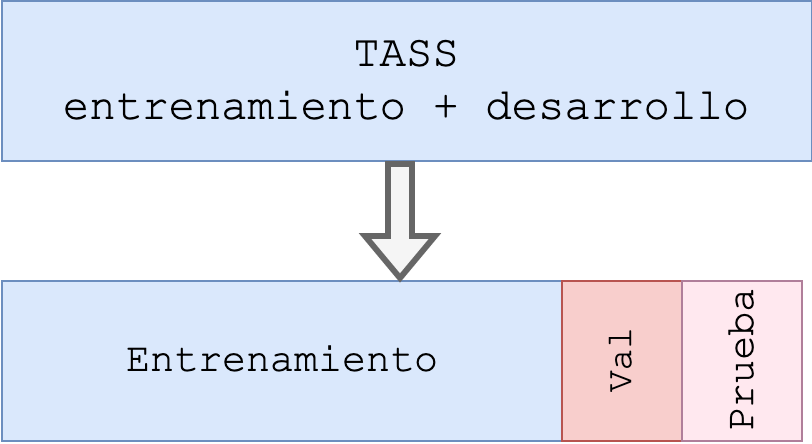
\includegraphics[keepaspectratio,width=0.4\textwidth]{./img/comia_blue_particion.png}
\caption{\label{fig:particiones}Particiones sobre el dataset TASS.}
\end{figure}

Se realizaron dos tipos de experimentos, cada uno de ellos utilizando los 3
modelos seleccionados, para las 4 configuraciones de datos descritas en
la Sección \ref{sec:preproceso}.

En el primer experimento se utiliza la partición de entrenamiento para entrenar
al modelo como pseudoetiquetador. En primera instancia, mediante un proceso
inspirado en \emph{k-fold cross validation}, se eliminan las etiquetas de un
porcentaje de los datos de entrenamiento (variando en cada iteración los datos
a los cuales se les quitó su etiqueta); posteriormente se entrena al modelo con
los datos que aún mantienen su etiqueta verdadera; toda vez que se ha entrenado
al modelo, se procede a asignar etiquetas a los datos que carecen de ellas, aquí
se conservan los \(k\) mejores resultados para reentrenar el modelo con los datos
con etiquetas verdaderas y los nuevos \(k\) datos, este proceso continúa hasta
terminar de asignar nuevas etiquetas; por último, se utiliza el conjunto de
validación (\Cref{fig:particiones}) para medir el desempeño del modelo, tanto como
pseudoetiquetador y como clasificador al final del experimento. La \Cref{fig:exp1}
muestra el procedimiento llevado a cabo.

\begin{figure}[htbp!]
\centering
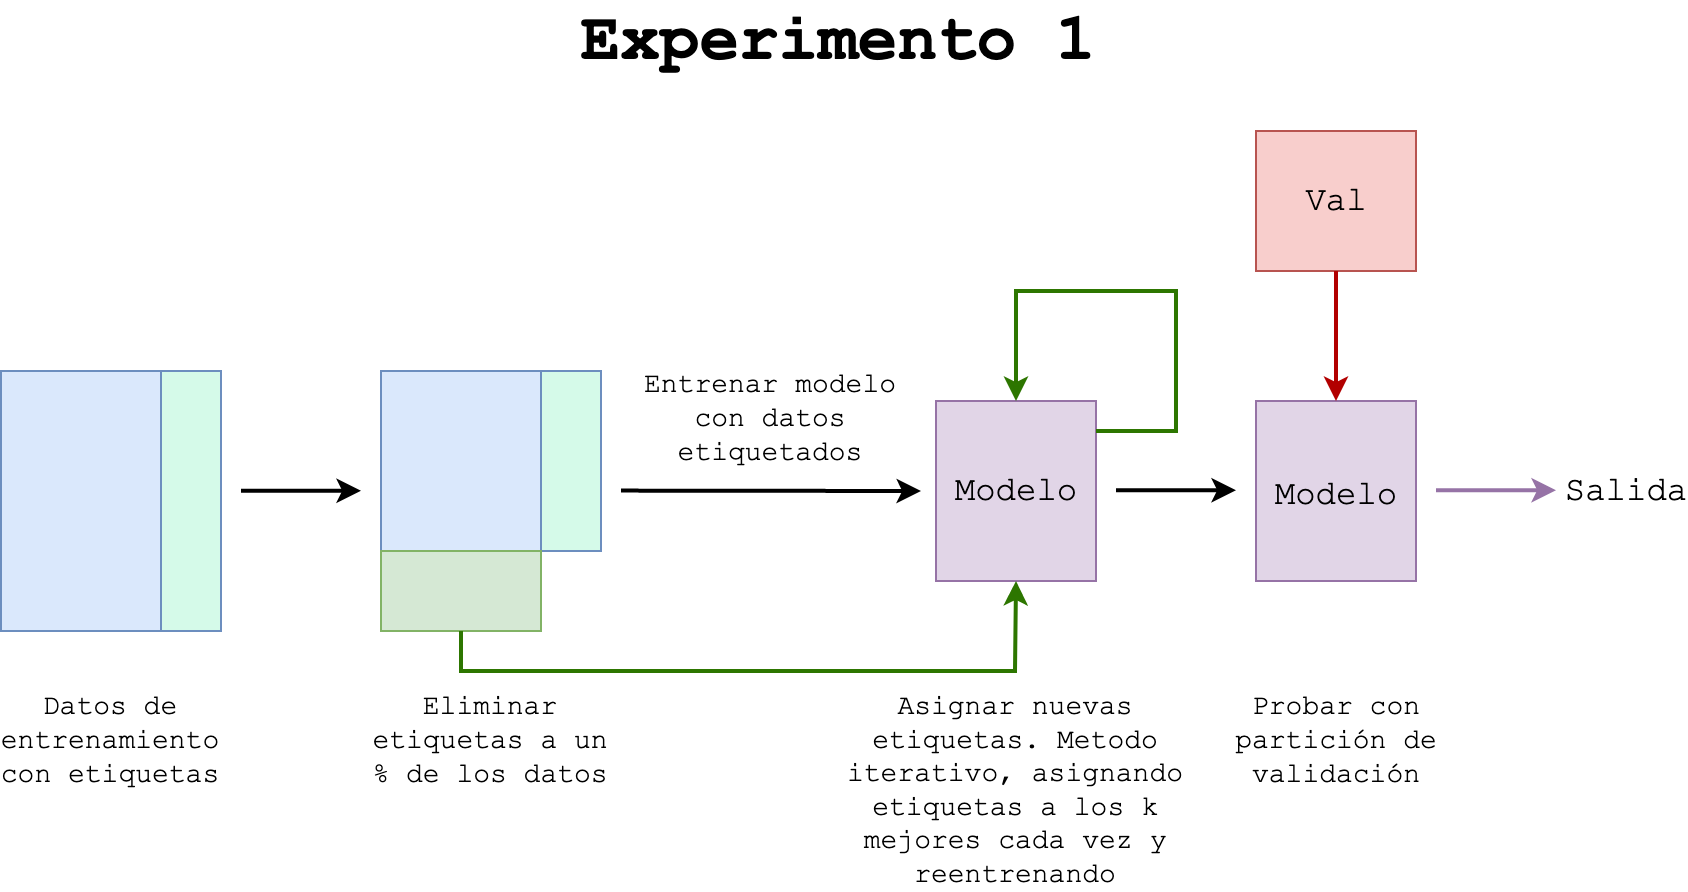
\includegraphics[keepaspectratio,width=\textwidth]{./img/comia_blue_exp1.png}
\caption{\label{fig:exp1}Experimento 1.}
\end{figure}

En el segundo experimento se vuelve a trabajar con el conjunto de entrenamiento
para utilizar al modelo como pseudoetiquetador, una vez que se ha entrenado,
se procede a añadir etiquetas a los datos extraídos de Twitter (que no tienen
una etiqueta asignada) mediante el mismo proceso del experimento 1, es decir,
se asignan etiquetas a todos los datos, se conservan las \(k\) mejores para
reentrenar al modelo y así sucesivamente, hasta terminar de etiquetar los datos
de Twitter. Una vez que se ha concluído esa primera etapa, se procede a medir
el desmepeño del modelo con el conjunto de prueba (\Cref{fig:particiones}). De
igual modo, la \Cref{fig:exp2} muestra el procedimiento realizado en el
experimento 2.

\begin{figure}[htbp!]
\centering
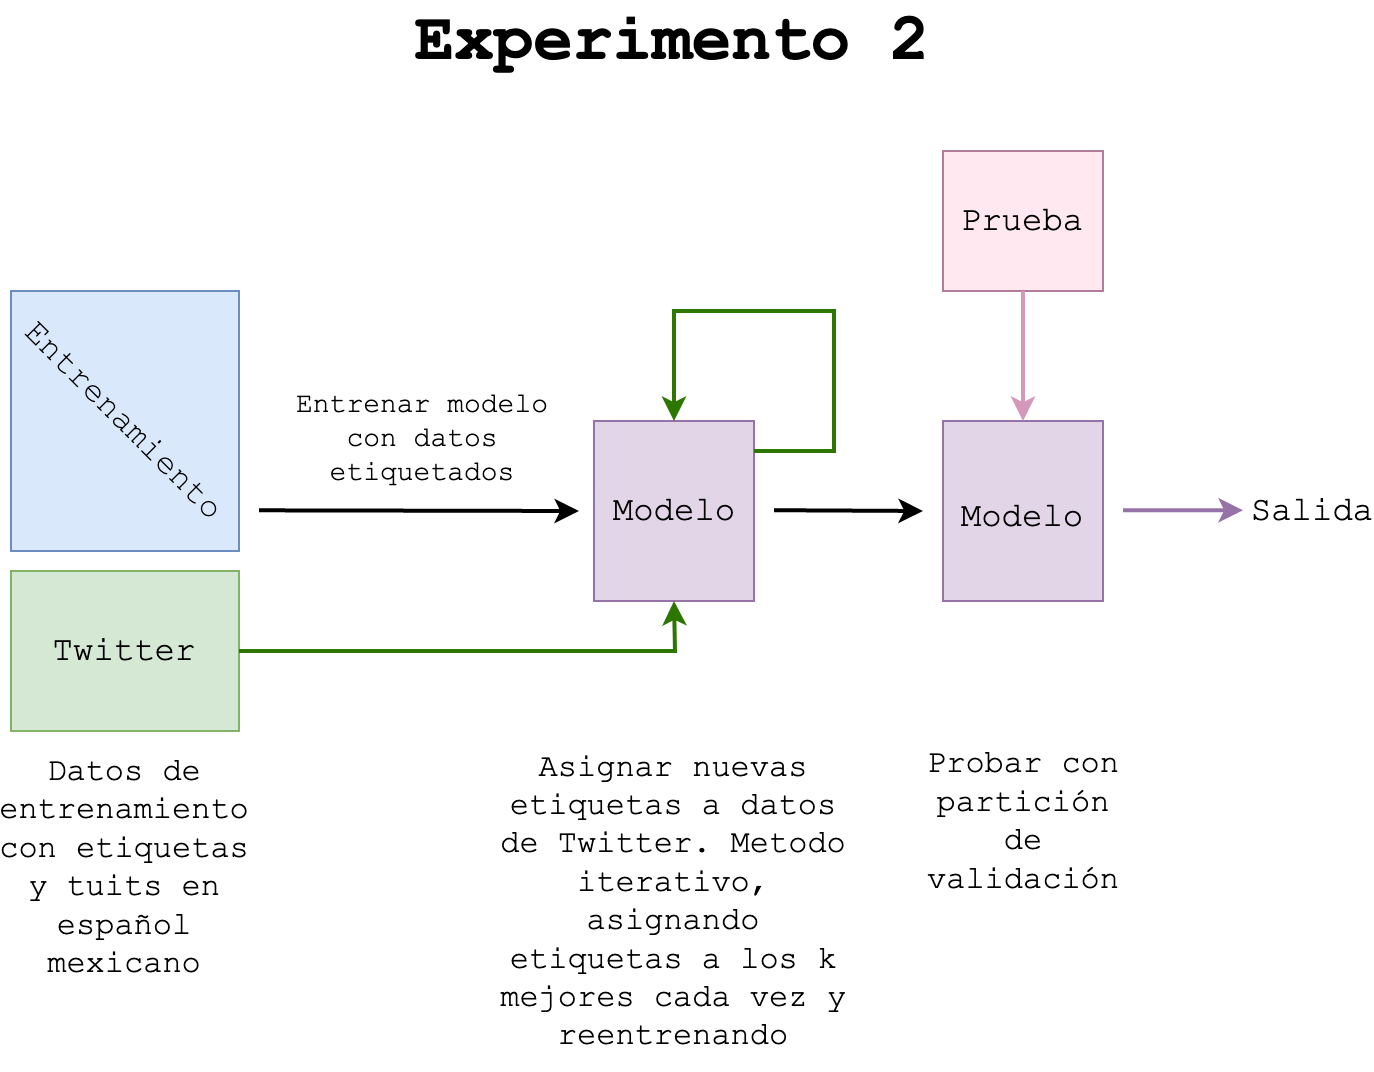
\includegraphics[keepaspectratio,width=0.82\textwidth]{./img/comia_blue_exp2.png}
\caption{\label{fig:exp2}Experimento 2.}
\end{figure}
\clearpage


\section{Resultados}
\label{sec:org2db8ff9}
En esta sección se presentan los resultados de ambos experimentos. En las
tablas \ref{tab:exp_1_rl,tab:exp_1_svm,tab:exp_1_nbm} se muestran los resultados
obtenidos en el experimento 1 con los modelos RL, SVM y NBM, respectivamente.

\begin{table}[htbp!]
\centering
\caption{Resultados del experimento 1 con el modelo de RL}
\label{tab:exp_1_rl}
\resizebox{\textwidth}{!}{%
\begin{tabular}{crrrrrr}
\hline
Configuración      & \% ignorado & cantidad train & Recall          & Precisión       & Acc             & F1              \\ \hline
\multirow{5}{*}{1} & 0           & 1050           & 0.4981          & 0.5018          & 0.5822          & 0.4992          \\
                   & \textbf{20} & \textbf{}      & \textbf{0.5297} & \textbf{0.5493} & \textbf{0.6151} & \textbf{0.5341} \\
                   & 40          & 1050           & 0.5028          & 0.5142          & 0.5813          & 0.5048          \\
                   & 60          & 1050           & 0.4829          & 0.4982          & 0.584           & 0.4825          \\
                   & 80          & 1050           & 0.4222          & 0.437           & 0.584           & 0.4094          \\ \hline
\multirow{5}{*}{2} & \textbf{0}  & \textbf{1050}  & \textbf{0.4992} & \textbf{0.49}   & \textbf{0.5644} & \textbf{0.4557} \\
                   & 20          & 1050           & 0.4316          & 0.4777          & 0.544           & 0.4287          \\
                   & 40          & 1050           & 4339            & 0.4589          & 0.5333          & 0.4293          \\
                   & 60          & 1050           & 0.4288          & 0.4742          & 0.5458          & 0.4191          \\
                   & 80          & 1050           & 0.4038          & 0.4383          & 0.5124          & 0.3824          \\ \hline
\multirow{5}{*}{3} & \textbf{0}  & \textbf{1050}  & \textbf{0.5262} & \textbf{0.5469} & \textbf{0.6044} & \textbf{0.5326} \\
                   & 20          & 1050           & 0.5105          & 0.5212          & 0.5884          & 0.5137          \\
                   & 40          & 1050           & 0.5036          & 0.5231          & 0.5862          & 0.5079          \\
                   & 60          & 1050           & 0.4696          & 0.4908          & 0.5644          & 0.4694          \\
                   & 80          & 1050           & 0.421           & 0.4607          & 0.5378          & 0.4076          \\ \hline
\multirow{5}{*}{4} & 0           & 1050           & 0.4731          & 0.4771          & 0.5422          & 0.4747          \\
                   & \textbf{20} & \textbf{1050}  & \textbf{0.4953} & \textbf{0.5005} & \textbf{0.5667} & \textbf{0.4958} \\
                   & 40          & 1050           & 0.4809          & 0.4878          & 0.5596          & 0.4815          \\
                   & 60          & 1050           & 0.4539          & 0.4662          & 0.5489          & 0.4544          \\
                   & 80          & 1050           & 0.4284          & 0.434           & 0.5307          & 0.4212          \\ \hline
\end{tabular}%
}
\end{table}

\begin{table}[htbp!]
\centering
\caption{Resultados del experimento 1 con el modelo de SVM}
\label{tab:exp_1_svm}
\resizebox{\textwidth}{!}{%
\begin{tabular}{crrrrr}
\hline
Configuración      & \% ignorado & Recall          & Precisión       & Acc             & F1              \\ \hline
\multirow{5}{*}{1} & 0           & 0.5039          & 0.5899          & .6444           & 0.4949          \\
                   & \textbf{20} & \textbf{0.526}  & \textbf{0.5379} & \textbf{0.6049} & \textbf{0.5291} \\
                   & 40          & 0.4979          & 0.5104          & 0.5884          & 0.4989          \\
                   & 60          & 0.4758          & 0.4952          & 0.5778          & 0.4749          \\
                   & 80          & 0.4275          & 0.4484          & 0.5449          & 0.4187          \\ \hline
\multirow{5}{*}{2} & \textbf{0}  & \textbf{0.4538} & \textbf{0.6328} & \textbf{0.5956} & \textbf{0.4448} \\
                   & 20          & 0.4416          & 0.4913          & 0.5547          & 0.4371          \\
                   & 40          & 0.4317          & 0.4821          & 0.536           & 0.4237          \\
                   & 60          & 0.4312          & 0.4545          & 0.5422          & 0.4222          \\
                   & 80          & 0.4078          & 0.4428          & 0.5302          & 0.3874          \\ \hline
\multirow{5}{*}{3} & 0           & 0.4764          & 0.7902          & 0.6311          & 0.4601          \\
                   & \textbf{20} & \textbf{0.5211} & \textbf{0.5388} & \textbf{0.5969} & \textbf{0.5259} \\
                   & 40          & 0.5049          & 0.5187          & 0.5827          & 0.508           \\
                   & 60          & 0.4872          & 0.521           & 0.5756          & 0.4918          \\
                   & 80          & 0.4291          & 0.4786          & 0.5471          & 0.4224          \\ \hline
\multirow{5}{*}{4} & \textbf{0}  & \textbf{0.4901} & \textbf{0.6983} & \textbf{0.6356} & \textbf{0.4822} \\
                   & 20          & 0.4794          & 0.4848          & 0.5591          & 0.4804          \\
                   & 40          & 0.4761          & 0.489           & 0.5578          & 0.4764          \\
                   & 60          & 0.4535          & 0.4679          & 0.5418          & 0.4535          \\
                   & 80          & 0.4326          & 0.4592          & 0.5329          & 0.4279          \\ \hline
\end{tabular}%
}
\end{table}

\begin{table}[htbp!]
\centering
\caption{Resultados del experimento 1 con el modelo de NBM}
\label{tab:exp_1_nbm}
\resizebox{\textwidth}{!}{%
\begin{tabular}{crrrrr}
\hline
Configuración      & \multicolumn{1}{l}{\% ignorado} & \multicolumn{1}{l}{Recall}          & \multicolumn{1}{l}{Precisión}       & \multicolumn{1}{l}{Acc}             & \multicolumn{1}{l}{F1}              \\ \hline
\multirow{5}{*}{1} & \textbf{0}                      & \textbf{0.4883}                     & \textbf{0.4883}                     & \textbf{0.4883}                     & \textbf{0.4883}                     \\
                   & 20                              & 0.4589                              & 0.455                               & 0.6244                              & 0.4235                              \\
                   & 40                              & 0.4356                              & 0.4882                              & 0.6031                              & 0.3964                              \\
                   & 60                              & 0.4001                              & 0.4511                              & 0.5707                              & 0.3455                              \\
                   & 80                              & 0.3498                              & 0.4344                              & 0.5218                              & 0.2604                              \\ \hline
\multirow{5}{*}{2} & \multicolumn{1}{l}{\textbf{0}}  & \multicolumn{1}{l}{\textbf{0.4883}} & \multicolumn{1}{l}{\textbf{0.5459}} & \multicolumn{1}{l}{\textbf{0.5956}} & \multicolumn{1}{l}{\textbf{0.4406}} \\
                   & \multicolumn{1}{l}{20}          & \multicolumn{1}{l}{0.4502}          & \multicolumn{1}{l}{0.5855}          & \multicolumn{1}{l}{0.5973}          & \multicolumn{1}{l}{0.4343}          \\
                   & \multicolumn{1}{l}{40}          & \multicolumn{1}{l}{0.4271}          & \multicolumn{1}{l}{0.5129}          & \multicolumn{1}{l}{0.5836}          & \multicolumn{1}{l}{0.3969}          \\
                   & \multicolumn{1}{l}{60}          & \multicolumn{1}{l}{0.4137}          & \multicolumn{1}{l}{0.4854}          & \multicolumn{1}{l}{0.5764}          & \multicolumn{1}{l}{0.3723}          \\
                   & \multicolumn{1}{l}{80}          & \multicolumn{1}{l}{0.3856}          & \multicolumn{1}{l}{0.4493}          & \multicolumn{1}{l}{0.5551}          & \multicolumn{1}{l}{0.3245}          \\ \hline
\multirow{5}{*}{3} & \textbf{0}                      & \textbf{0.5539}                     & \textbf{0.624}                      & \textbf{0.6667}                     & \textbf{0.5608}                     \\
                   & 20                              & 0.5201                              & 0.6097                              & 0.648                               & 0.5127                              \\
                   & 40                              & 0.5099                              & 0.5996                              & 0.644                               & 0.4969                              \\
                   & 60                              & 0.4671                              & 0.5786                              & 0.6076                              & 0.448                               \\
                   & 80                              & 0.4327                              & 0.4582                              & 0.5636                              & 0.3937                              \\ \hline
\multirow{5}{*}{4} & \textbf{0}                      & \textbf{0.5341}                     & \textbf{0.6427}                     & \textbf{0.6578}                     & \textbf{0.5388}                     \\
                   & 20                              & 0.5159                              & 0.6908                              & 0.6498                              & 0.5131                              \\
                   & 40                              & 0.4913                              & 0.6497                              & 0.6329                              & 0.4772                              \\
                   & 60                              & 0.4751                              & 0.6585                              & 0.6147                              & 0.457                               \\
                   & 80                              & 0.3765                              & 0.5051                              & 0.5391                              & 0.3169                              \\ \hline
\end{tabular}%
}
\end{table}

Por su parte, las tablas \ref{tab:exp_2_rl,tab:exp_2_svm,tab:exp_2_nbm} muestran los
resultados obtenidos en el experimento 2 con los modelos RL, SVM y NBM,
respectivamente.
\begin{table}[htbp!]
\centering
\caption{Resultados del experimento 2 con el modelo de RL}
\label{tab:exp_2_rl}
\resizebox{\textwidth}{!}{%
\begin{tabular}{crrrrrrrr}
\hline
\multicolumn{1}{l}{Configuración} & \% pseudo   & Total         & Orig          & Pseudo       & Recall          & Precisión       & Acc             & F1              \\ \hline
\multirow{5}{*}{1}                & 0           & 1050          & 1050          & 0            & 0.5403          & 0.5526          & 0.6267          & 0.5405          \\
                                  & 20          & 1312          & 1050          & 263          & 0.5404          & 0.5682          & 0.6262          & 0.5440          \\
                                  & \textbf{40} & \textbf{1749} & \textbf{1050} & \textbf{700} & \textbf{0.5516} & \textbf{0.5764} & \textbf{0.6324} & \textbf{0.5557} \\
                                  & 60          & 2623          & 1050          & 1574         & 0.5451          & 0.5694          & 0.6248          & 0.5484          \\
                                  & 80          & 5245          & 1050          & 4196         & 0.5495          & 0.5774          & 0.6328          & 0.5532          \\ \hline
\multirow{5}{*}{2}                & \textbf{0}  & \textbf{1050} & \textbf{1050} & \textbf{0}   & \textbf{0.4217} & \textbf{0.4474} & \textbf{0.5333} & \textbf{0.4079} \\
                                  & 20          & 1312          & 1050          & 263          & 0.3642          & 0.4583          & 0.508           & 0.3035          \\
                                  & 40          & 1749          & 1050          & 700          & 0.3623          & 0.4656          & 0.5075          & 0.2955          \\
                                  & 60          & 2623          & 1050          & 1574         & 0.3656          & 0.4369          & 0.5106          & 0.3013          \\
                                  & 80          & 5245          & 1050          & 4196         & 0.3662          & 0.4571          & 0.5111          & 0.3033          \\ \hline
\multirow{5}{*}{3}                & 0           & 1050          & 1050          & 0            & 0.5034          & 0.507           & 0.5867          & 0.5021          \\
                                  & 20          & 1312          & 1050          & 263          & 0.5226          & 0.5484          & 0.6004          & 0.5273          \\
                                  & \textbf{40} & \textbf{1749} & \textbf{1050} & \textbf{700} & \textbf{0.5296} & \textbf{0.5471} & \textbf{0.604}  & \textbf{0.533}  \\
                                  & 60          & 2623          & 1050          & 1574         & 0.528           & 0.5495          & 0.6062          & 0.5315          \\
                                  & 80          & 5245          & 1050          & 4196         & 0.5248          & 0.545           & 0.6027          & 0.5279          \\ \hline
\multirow{5}{*}{4}                & \textbf{0}  & \textbf{1050} & \textbf{1050} & \textbf{0}   & \textbf{0.5155} & \textbf{0.5313} & \textbf{0.5956} & \textbf{0.5177} \\
                                  & 20          & 1312          & 1050          & 263          & 0.4913          & 0.5016          & 0.5796          & 0.4894          \\
                                  & 40          & 1749          & 1050          & 700          & 0.4864          & 0.4979          & 0.5733          & 0.4843          \\
                                  & 60          & 2623          & 1050          & 1574         & 0.4818          & 0.4935          & 0.5702          & 0.4803          \\
                                  & 80          & 5245          & 1050          & 4196         & 0.4919          & 0.5007          & 0.58            & 0.4885          \\ \hline
\end{tabular}%
}
\end{table}

\begin{table}[htbp!]
\centering
\caption{Resultados del experimento 2 con el modelo de SVM}
\label{tab:exp_2_svm}
\resizebox{\textwidth}{!}{%
\begin{tabular}{crrrrrrrr}
\hline
\multicolumn{1}{c}{Configuración} & \multicolumn{1}{r}{\% pseudo} & \multicolumn{1}{r}{Total} & \multicolumn{1}{r}{Orig} & \multicolumn{1}{r}{Pseudo} & \multicolumn{1}{r}{Recall} & \multicolumn{1}{r}{Precisión} & \multicolumn{1}{r}{Acc} & \multicolumn{1}{r}{F1} \\ \hline
\multirow{5}{*}{1}              & 0                             & 1050                      & 1050                     & 0                          & 0.4938                     & 0.7688                        & 0.6311                  & 0.4599                 \\
                                & 20                            & 1312                      & 1050                     & 263                        & 0.4979                     & 0.7707                        & 0.6329                  & 0.4706                 \\
                                & \textbf{40}                   & \textbf{1749}             & \textbf{1050}            & \textbf{700}               & \textbf{0.4988}            & \textbf{0.7713}               & \textbf{0.6342}         & \textbf{0.4713}        \\
                                & 60                            & 2623                      & 1050                     & 1574                       & 0.4933                     & 0.7684                        & 0.6307                  & 0.4595                 \\
                                & 80                            & 5245                      & 1050                     & 4196                       & 0.4938                     & 0.7688                        & 0.6311                  & 0.4599                 \\ \hline
\multirow{5}{*}{2}              & \textbf{0}                    & \textbf{1050}             & \textbf{1050}            & \textbf{0}                 & \textbf{0.4135}            & \textbf{0.4816}               & \textbf{0.5644}         & \textbf{0.3692}        \\
                                & 20                            & 1312                      & 1050                     & 263                        & 0.3904                     & 0.4629                        & 0.5458                  & 0.3282                 \\
                                & 40                            & 1749                      & 1050                     & 700                        & 0.4054                     & 0.4742                        & 0.56                    & 0.3512                 \\
                                & 60                            & 2623                      & 1050                     & 1574                       & 0.4096                     & 0.471                         & 0.5627                  & 0.3591                 \\
                                & 80                            & 5245                      & 1050                     & 4196                       & 0.415                      & 0.4729                        & 0.5667                  & 0.3689                 \\ \hline
\multirow{5}{*}{3}              & \textbf{0}                    & \textbf{1050}             & \textbf{1050}            & \textbf{0}                 & \textbf{0.4652}            & \textbf{0.7853}               & \textbf{0.6089}         & \textbf{0.4335}        \\
                                & 20                            & 1312                      & 1050                     & 263                        & 0.4613                     & 0.619                         & 0.6067                  & 0.4258                 \\
                                & 40                            & 1749                      & 1050                     & 700                        & 0.4617                     & 0.6507                        & 0.6067                  & 0.4265                 \\
                                & 60                            & 2623                      & 1050                     & 1574                       & 0.4648                     & 0.785                         & 0.6084                  & 0.433                  \\
                                & 80                            & 5245                      & 1050                     & 4196                       & 0.4652                     & 0.7853                        & 0.6089                  & 0.4335                 \\ \hline
\multirow{5}{*}{4}              & \textbf{0}                    & \textbf{1050}             & \textbf{1050}            & \textbf{0}                 & \textbf{0.4592}            & \textbf{0.4278}               & \textbf{0.6044}         & \textbf{0.4174}        \\
                                & 20                            & 1312                      & 1050                     & 263                        & 0.4587                     & 0.4274                        & 0.604                   & 0.4169                 \\
                                & 40                            & 1749                      & 1050                     & 700                        & 0.4587                     & 0.4274                        & 0.604                   & 0.4169                 \\
                                & 60                            & 2623                      & 1050                     & 1574                       & 0.4592                     & 0.4278                        & 0.6044                  & 0.4174                 \\
                                & 80                            & 5245                      & 1050                     & 4196                       & 0.4592                     & 0.4278                        & 0.6044                  & 0.4174                 \\ \hline
\end{tabular}%
}
\end{table}

\begin{table}[htbp!]
\centering
\caption{Resultados del experimento 2 con el modelo de NBM}
\label{tab:exp_2_nbm}
\begin{tabular}{crrrrrrrr}
\hline
\multicolumn{1}{c}{Configuración} & \multicolumn{1}{r}{\% pseudo} & \multicolumn{1}{r}{Total} & \multicolumn{1}{r}{Orig} & \multicolumn{1}{r}{Pseudo} & \multicolumn{1}{r}{Recall} & \multicolumn{1}{r}{Precisión} & \multicolumn{1}{r}{Acc} & \multicolumn{1}{r}{F1} \\ \hline
\multirow{5}{*}{1}              & \textbf{0}                    & \textbf{1050}             & \textbf{1050}            & \textbf{0}                 & \textbf{0.461}             & \textbf{0.5766}               & \textbf{0.5956}         & \textbf{0.4343}        \\
                                & 20                            & 1312                      & 1050                     & 263                        & 0.4569                     & 0.665                         & 0.5964                  & 0.4277                 \\
                                & 40                            & 1749                      & 1050                     & 700                        & 0.4356                     & 0.533                         & 0.5844                  & 0.3921                 \\
                                & 60                            & 2623                      & 1050                     & 1574                       & 0.4211                     & 0.4577                        & 0.5733                  & 0.3727                 \\
                                & 80                            & 5245                      & 1050                     & 4196                       & 0.3962                     & 0.4833                        & 0.5516                  & 0.3365                 \\ \hline
\multirow{5}{*}{2}              & \textbf{0}                    & \textbf{1050}             & \textbf{1050}            & \textbf{0}                 & \textbf{0.3858}            & \textbf{0.4469}               & \textbf{0.5289}         & \textbf{0.3372}        \\
                                & 20                            & 1312                      & 1050                     & 263                        & 0.3366                     & 0.3983                        & 0.4964                  & 0.2272                 \\
                                & 40                            & 1749                      & 1050                     & 700                        & 0.3333                     & 0.1644                        & 0.4933                  & 0.2202                 \\
                                & 60                            & 2623                      & 1050                     & 1574                       & 0.3333                     & 0.1644                        & 0.4933                  & 0.2202                 \\
                                & 80                            & 5245                      & 1050                     & 4196                       & 0.3333                     & 0.1644                        & 0.4933                  & 0.2202                 \\ \hline
\multirow{5}{*}{3}              & \textbf{0}                    & \textbf{1050}             & \textbf{1050}            & \textbf{0}                 & \textbf{0.4981}            & \textbf{0.5527}               & \textbf{0.6044}         & \textbf{0.4874}        \\
                                & 20                            & 1312                      & 1050                     & 263                        & 0.4908                     & 0.5452                        & 0.5982                  & 0.4824                 \\
                                & 40                            & 1749                      & 1050                     & 700                        & 0.4738                     & 0.5413                        & 0.5902                  & 0.457                  \\
                                & 60                            & 2623                      & 1050                     & 1574                       & 0.4638                     & 0.5367                        & 0.5916                  & 0.4384                 \\
                                & 80                            & 5245                      & 1050                     & 4196                       & 0.4506                     & 0.5183                        & 0.5871                  & 0.4143                 \\ \hline
\multirow{5}{*}{4}              & 0                             & 1050                      & 1050                     & 0                          & 0.4608                     & 0.4934                        & 0.5778                  & 0.4347                 \\
                                & \textbf{20}                   & \textbf{1312}             & \textbf{1050}            & \textbf{263}               & \textbf{0.4679}            & \textbf{0.5188}               & \textbf{0.5849}         & \textbf{0.4447}        \\
                                & 40                            & 1749                      & 1050                     & 700                        & 0.4615                     & 0.5085                        & 0.588                   & 0.4288                 \\
                                & 60                            & 2623                      & 1050                     & 1574                       & 0.4571                     & 0.5472                        & 0.5924                  & 0.4196                 \\
                                & 80                            & 5245                      & 1050                     & 4196                       & 0.4505                     & 0.4724                        & 0.592                   & 0.4102                 \\ \hline
\end{tabular}%
\end{table}

\clearpage
\section{Conclusiones}
\label{sec:org58ea8f4}
Conclusiones

\section{Referencias}
\label{sec:org856da34}
\printbibliography
\end{document}